% !TeX root = ../main.tex
% Add the above to each chapter to make compiling the PDF easier in some editors.

\chapter{Feintypen nach GDV}\label{chapter:Anhang1}

Für die Typisierung der Unfälle werden die Unfalltypen der GDV verwendet. Diese sind gut geeignet, da die sieben Unfalltypen in weitere Feintypen unterteilt wurden. Zur besseren Verständlichkeit werden die einzelnen Feintypen in den Abbildungen \ref{fig:FT1} bis \ref{fig:FT7} dargestellt. %Text evtl. weglassen, dann ist die Seite nicht fast leer.

\begin{savenotes}
	\begin{figure}[H]
		\centering
		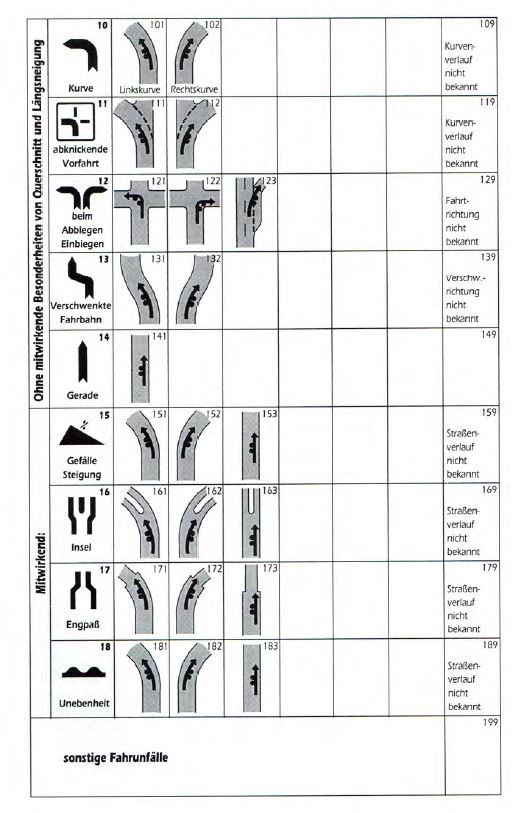
\includegraphics[width=13cm,height=21cm]{figures/FT1}
		\caption[Fahrunfall nach GDV]{Fahrunfall \parencite[S. 9]{GesamtverbandderDeutschenVersicherungswirtschafte.V..2016}. }\label{fig:FT1}
	\end{figure}
\end{savenotes}

\begin{savenotes}
	\begin{figure}[H]
		\centering
		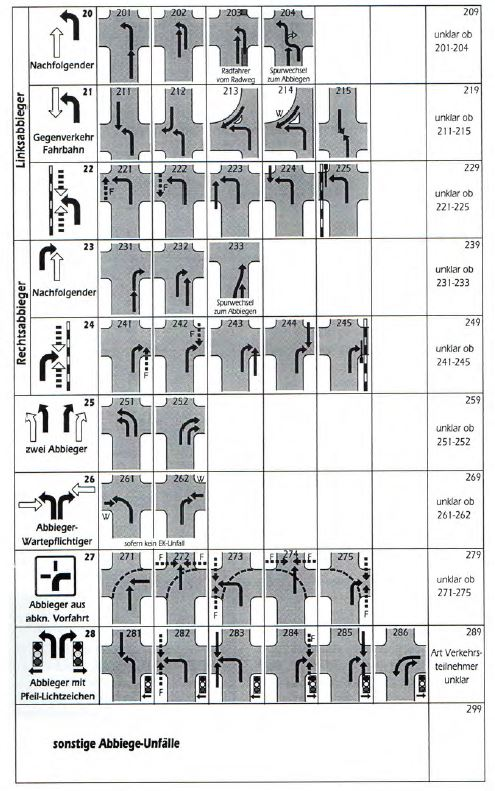
\includegraphics[width=13cm,height=21cm]{figures/FT2}
		\caption[Abbiege-Unfall nach GDV]{Abbiege-Unfall \parencite[S. 11]{GesamtverbandderDeutschenVersicherungswirtschafte.V..2016}. }\label{fig:FT2}
	\end{figure}
\end{savenotes}

\begin{savenotes}
	\begin{figure}[H]
		\centering
		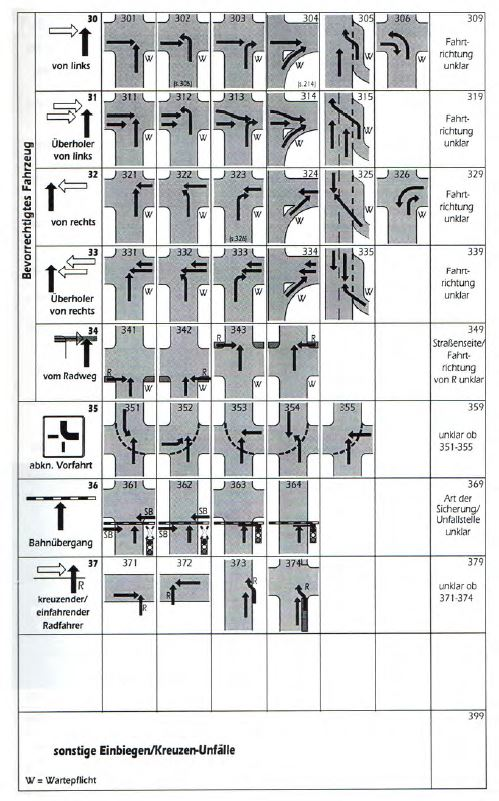
\includegraphics[width=13cm,height=21cm]{figures/FT3}
		\caption[Einbiegen/Kreuzen-Unfall nach GDV]{Einbiegen/Kreuzen-Unfall \parencite[S. 13]{GesamtverbandderDeutschenVersicherungswirtschafte.V..2016}. }\label{fig:FT3}
	\end{figure}
\end{savenotes}

\begin{savenotes}
	\begin{figure}[H]
		\centering
		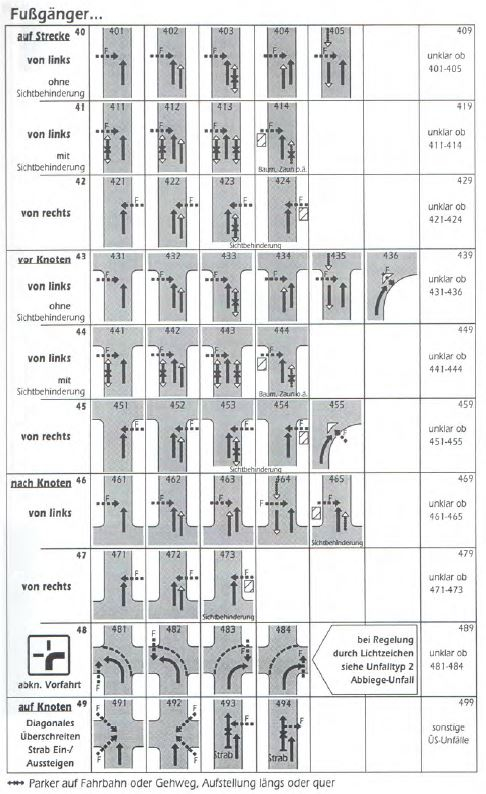
\includegraphics[width=13cm,height=21cm]{figures/FT4}
		\caption[Überschreiten-Unfall nach GDV]{Überschreiten-Unfall \parencite[S. 15]{GesamtverbandderDeutschenVersicherungswirtschafte.V..2016}. }\label{fig:FT4}
	\end{figure}
\end{savenotes}

\begin{savenotes}
	\begin{figure}[H]
		\centering
		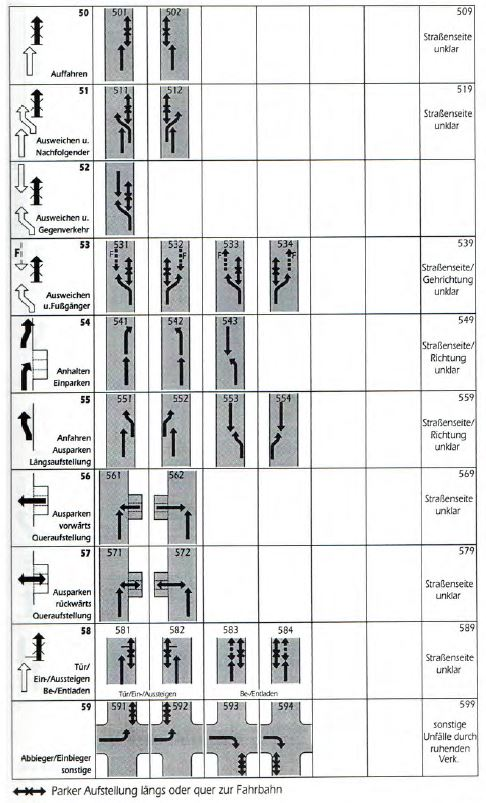
\includegraphics[width=13cm,height=21cm]{figures/FT5}
		\caption[Unfall durch ruhenden Verkehr nach GDV]{Unfall durch ruhenden Verkehr \parencite[S. 17]{GesamtverbandderDeutschenVersicherungswirtschafte.V..2016}. }\label{fig:FT5}
	\end{figure}
\end{savenotes}

\begin{savenotes}
	\begin{figure}[H]
		\centering
		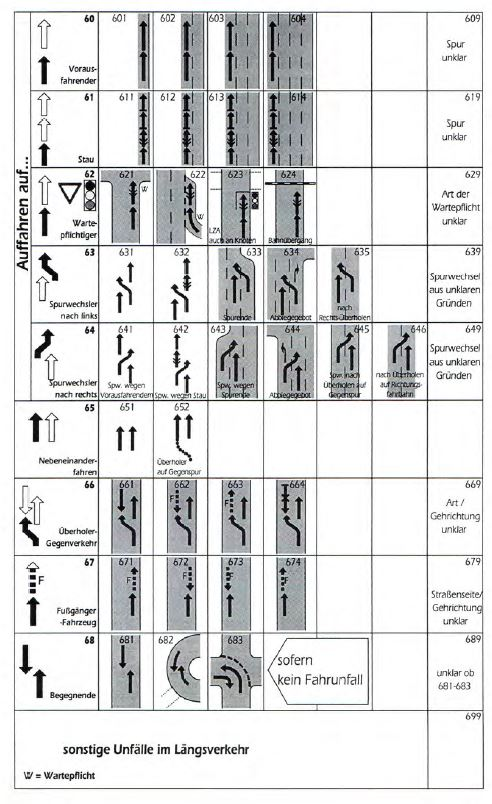
\includegraphics[width=13cm,height=21cm]{figures/FT6}
		\caption[Unfall im Längsverkehr nach GDV]{Unfall im Längsverkehr \parencite[S. 19]{GesamtverbandderDeutschenVersicherungswirtschafte.V..2016}. }\label{fig:FT6}
	\end{figure}
\end{savenotes}

\begin{savenotes}
	\begin{figure}[H]
		\centering
		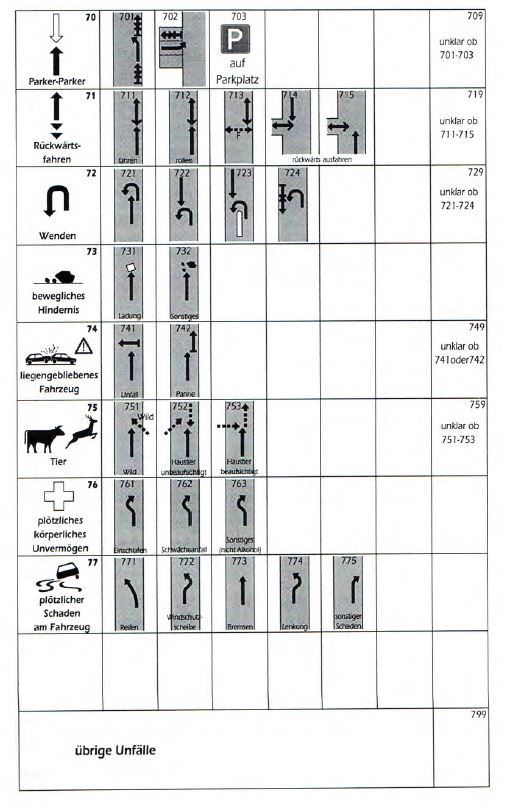
\includegraphics[width=13cm,height=21cm]{figures/FT7}
		\caption[Sonstiger Unfall nach GDV]{Sonstiger Unfall \parencite[S. 21]{GesamtverbandderDeutschenVersicherungswirtschafte.V..2016}. }\label{fig:FT7}
	\end{figure}
\end{savenotes}

